\mysubsection{Fabian Gärtner}{Development Hardware und Software}

Da die VR One von Zeiss mit ihrem Sichtfenster die Möglichkeit bietet, mittels der Kamera des Smartphones auch die Umgebung zu filmen und aus den in den vorigen Kapiteln genannten Gründen, sollte neben der eigentlichen VR-Anwendung auch eine Art AR-Interaktion zum Einsatz kommen, um das Spiel interessanter zu gestalten. Zum einen geschieht das dadurch, wie in den vorigen Kapiteln beschrieben, dass der Spieler zunächst die Realität über das Kamerabild sieht und schließlich über eine Art Wurmloch in das Spiel teleportiert wird, zum anderen durch die Bewegung in der virtuellen Welt mittels Bewegung eines Würfels in der echten Realität. Im Grunde wird hier also nicht die echte Realität, sondern die virtuelle Realität erweitert. Da es aber während des GameJams nicht möglich war, einen solchen Controller zur Steuerung in der Spielwelt mit Lagesensoren herzustellen, musste eine Möglichkeit gefunden werden, einzelne Seiten des Würfels lediglich mittels der zur Verfügung stehenden Smartphone-Kamera zu unterscheiden. In der Regel und auch bei inCubed geschieht eine solche Unterscheidung mittels verschiedener Marker. Solche Marker können in Form von QR-Codes, Bildern und anderen Strukturen gestaltet sein, erfordern dann allerdings eine Vielzahl an komplexen Algorithmen, um eine möglichst fehlerfreie Erkennung zu gewährleisten. In Anbetracht, dass für den Game Jam aber lediglich eine begrenzte Zeit zur Verfügung stand, wurde in einem iterativen Prozess eine andere Art an Markern gesucht, die eine sehr einfache und effiziente und denoch genaue und zuverlässige Erkennung ermöglichen. So war zunächst die Idee, die sechs Seiten des Würfels unterschiedlich einzufärben und/oder mittels schwarzen Linien unterscheidbar zu machen. Da Farbe allein allerdings anfällig für schlechte Lichtverhältnisse ist, zeigte sich bei Tests mit verschiedenen Würfel-Prototypen aus Papier, dass die Verwendung von geometrischen Formen als Marker zu deutlich besseren Ergebnissen führt. Daher kommen nun beim fertigen Controller die sechs Formen Kreis, Dreieck, Viereck, Pentagon, Heptagon und Stern zum Einsatz, wobei auf den gegenüberliegenden Seiten des Würfels jeweils zwei möglichst unterschiedliche Formen zu finden sind. Die Erkennung dieser Formen ist beim Prototypen von inCubed vollständig implementiert und bereits ausreichend, um auch unter schlechten Lichtverhältnissen eine korrekte Erkennung zu ermöglichen. Für das fertige Spiel kann aber noch auf zwei Redundanzinformationen zurückgegriffen werden: Gegenüberliegende Formen haben, auch aus designtechnischen Gründen (siehe \ref{Marker}) dieselbe Farbe, sodass mittels zusätzlicher Farberkennung die erkannte Form verifiziert werden kann. Des Weiteren ist jede Würfelseite mit einer dicken schwarzen Linie umrandet, sodass der Suchprozess nach Markern auf die Erkennung eines Quadrates und eine anschließende Formerkennung innerhalb des Quadrates unterteilt werden kann. Außerdem ist so bestimmbar, welche der Würfelseiten die größte Fläche im Kamerabild einnimmt, falls der Nutzer den Würfel nicht optimal hält und dadurch mehrere Formen erkennbar wären.

Programmiertechnisch wird zur effizienten Markererkennung die kostenfreie Open-Source-Bibliothek OpenCV verwendet, die die Anwendung von Algorithmen und grundlegenden mathematischen Operationen auf Matrizen und Bilder ermöglicht. OpenCV stellt Wrapper für verschiedene Plattformen zur Verfügung, u.a. auch für Java und Android. Zwar könnte mit Hilfe der ebenfalls kostenfreien Bibliothek EmguCV OpenCV auch direkt aus C\# angesteuert werden, da die Zielplattform allerdings ein Android-System ist, müssten dann die OpenCV-Systemdateien (.so auf Android statt .dll auf Windows) ausgetauscht werden, was zu Problemen führen könnte. Daher wurde für inCubed eine andere Variante gewählt: Die Erkennung selbst wird in einer selbstgeschriebenen Java-/Android-Bibliothek unter Verwendung von OpenCV for Android vorgenommen. Diese Bibliothek wird anschließend als .jar-Datei exportiert und in Unity als sogenanntes Android-Plugin angesteuert. Bevor näher auf diese Plugin-Mechanik und die aufgetretenen Probleme eingegangen wird, soll zunächst das Plugin selbst genauer beschrieben werden. Nach Laden von OpenCV (der OpenCV-Manager muss als App auf dem Smartphone vorinstalliert sein, das Plugin kann diese App dann in der von Android bekannten OnResume-Funktion oder zu einem späteren Zeitpunkt starten und verwenden), wird die Verbindung zur Smartphone-Kamera hergestellt und mittels Eventsystem so verknüpft, dass das Plugin über jedes von der Kamera aufgenommene Kamerabild informiert wird. In einem extra Thread wird dieses Kamerabild dann in mehreren Schritten mittels diverser Algorithmen weiterverarbeitet und für die Markererkennung vorbereitet.

Welche Algorithmen für eine Markererkennung genau verwendet werden ist vom Einzelfall abhängig, in der Regel aber hat sich eine Mischung aus Kanten- und Konturerkennung sowie einer anschließenden Polygonannäherung als Vorgehensweise etabliert. Diese Algorithmen werden auch von OpenCV zur Verfügung stellt. Konkret wird bei inCubed eine Mischung aus Gaußschem Weichzeichner, adaptivem Threshold und dem sogenannten Canny-Edge-Detektor verwendet, um aus dem Kamerabild eindeutige Konturen zu extrahieren. Diese werden dann mittels Konturerkennungs-Algorithmus exakt beschrieben und durch Reduktion und Glättung der erkannten Punkte an einfache Polygone angenähert. Letztlich muss anschließend nur noch aufgrund der Eckpunktanzahl, der Fläche, der Form (konvex oder konkav) und der Winkel der Kanten zueinander entschieden werden, um welche Form es sich handelt. So ist bspw. der Stern die einzige konkave Form, der Kreis hat eine besonders hohe Zahl an Eckpunkten und Pentagon und Heptagon unterscheiden sich sowohl durch die Eckpunktanzahl als auch durch ihre Innenwinkel. Das Ergebnis dieser Erkennung und die Position der Bounding Box der Form sowie das Kamerabild wird anschließend an die Unity-Anwendung übergeben und von inCubed selbst weiterverarbeitet. Es zeigt sich hier, dass dieser Bildverarbeitungsprozess zwar relativ zeitaufwändig ist (letztlich aber immer noch effizienter als bei andernen Markerarten), aber sehr zuverlässig arbeitet und auch in dunkleren Räumen noch fehlerfrei die unterschiedlichen Formen erkennen kann. Durch die oben genannten Redundanzen könnte die Erkennung aber dennoch weiter verbessert werden. Für eine spätere Version des Spiels wäre es zudem denkbar Sensoren im Würfel zu platzieren, die mittels Bluetooth ihre Lage im Raum an das Smartphone senden. Dann könnte die Markererkennung zur Kalibrierung eingesetzt werden. Schon jetzt wird der Spieler zu Beginn des Spiels gebeten den Stern in die Kamera zu halten, sodass ein Kalibrierungsmodus jederzeit nachimplementiert werden kann.

Hier kommt nun das Pluginsystem von Unity zum Einsatz. Bereits im Plugin selbst kann durch Einbindung einer von Unity bereitgestellten classes.jar auf Unity-Funktionalität zurückgegriffen werden. So ist es bspw., nachdem der Nutzer seine Android-Activity von der UnityPlayerActivity abgeleitet hat, möglich, Nachrichten mittels SendMessage an beliebige GameObjects zu senden. Um ein solches Plugin dann in einer konkreten Unity-Anwendung einzusetzen, muss das Plugin als .jar-Datei exportiert und zusammen mit einer modifizierten AndroidManifest.xml in den Ordner Assets/Plugins/Android/ des jeweiligen Projektes gelegt werden. Unity bindet das Plugin dadurch automatisch in die Anwendung mit ein und ermöglicht es so, die im Plugin definierte Funktionalität aus C\# aus aufzurufen. Ein solcher Auruf kann wie in \ref{fig:Code} aussehen, wobei hier die im Plugin als öffentliche Methode definierte Methode \enquote{GetShapePosition} aufgerufen wird und der Rückgabewert in einer Variable gespeichert wird.

\begin{figure}[!htbp]%[htbp]
	\centering
		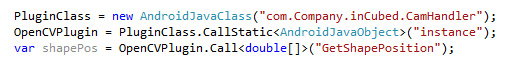
\includegraphics[width=1.0\textwidth]{images/code}
	\caption{Austausch von Daten zwischen Unity und dem Plugin}
	\label{fig:Code}
\end{figure}

Während dieses Pluginsystem durchaus Vorteile bietet und in inCubed auch zur Verwendung von Cardboard-Funktionalität zum Einsatz kommt, gibt es einige größere Nachteile, die die Entwicklung von inCubed zunächt beeinträchtigt haben. Die zur Verfügung stehenden Funktionalitäten sind zwar von Unity aus ausführlich dokumentiert (teilweise allerdings relativ unstrukturiert), in der Praxis waren aber dennoch viele schrittweise Tests erforderlich, um ein erstes lauffähiges Plugin zu implementieren. Gerade dadurch, dass ein selbstgeschriebenes Android-Manifest benötigt wird, dieses aber nicht ausführlich genug in der Doku erklärt wird, sind hier immer wieder Fehler aufgetreten. Des Weiteren gab es dadurch Probleme, dass auch das Cardboard-SDK als Android-Plugin ausgeliefert wird. Android selbst ist nicht dafür gemacht, dass mehrere Apps gleichzeitig aktiv sind. Es war daher zunächst nicht möglich sowohl VR- als auch AR-Funktionalität gleichzeitig einzusetzen. Dies führte zu Abstürzen von inCubed unter Ausgabe kryptischer Fehlermeldungen. Erst als dann das Cardboard-Plugin selbst durch die Funktionalität des selbstgeschriebenen Plugins erweitert und so letztlich nur noch ein Plugin benötigt wurde, war dieses Problem behoben. Aktuell ist nun hauptsächlich noch die Performance das größte Problem. Zwar liegt die Performance des Cardbord-Plugins als auch die Performance des selbstgeschrieben Markererkennungs-Plugins mit OpenCV auf dem verwendeten Samsung Galaxy S4 für sich genommen durchaus in einem vertretbarem Rahmen, arbeiten aber beide Plugins zusammen, zeigen sich größere Leistungseinbrüche. Dafür scheint es mehrere Gründe zu geben: zum einen ist das Galaxy S4 im Vergleich zu neueren Modellen nicht besonders leistungsstark, zum anderen verwendet Unity und OpenCV im Hintergrund ein Native Development Kit, um Funktionalität von Java nach C++ konvertieren zu können. Dies benötigt zusätzlich Leistung und Zeit, sodass es aktuell beim Intro und Outro von inCubed zu Performance-Einbrüchen kommt und das Kamerabild um etwa eine Sekunde verzöger angezeigt wird. Es ist davon auszugehen, dass sich auf einem Smartphone wie dem Samsung Galaxy S6, das auch mit der VR-One-Alternative GearVR ausgeliefert wird, solche Probleme deutlich weniger schwerwiegend auswirken sollten. Für einen Prototypen wie er während des Game Jams entstanden ist, ist die schlechte Performance aber verzeihbar.
